\documentclass{article}
\usepackage[margin=1in]{geometry} %1 in margins
\usepackage{graphicx} %For including graphics
\usepackage[labelfont=bf]{caption} %Make float labels bold
\usepackage{subcaption}
\usepackage{amsmath}    
\usepackage{listings}% http://ctan.org/pkg/listings
\usepackage{cancel}
\lstset{
  basicstyle=\ttfamily,
  mathescape
}
\usepackage{hyperref}
\renewcommand{\floatpagefraction}{0.95}
\renewcommand{\topfraction}{0.95}
\renewcommand{\textfraction}{0.05}
\usepackage{url}

% Define a ``Program'' float for code
\usepackage{verbatim} %Allow verbatim input for code
\usepackage{float} %Defining the Program environment
\floatstyle{boxed}
\newfloat{program}{htbp}{pgm}
\floatname{program}{Program}



\begin{document}

\begin{flushright}
	Mehmet Duman
\end{flushright}

\begin{center}
{\Large {\bf Solution to Homework \#7---MTH 522} }
\end{center}

{\bf Problem 1} (Chapter 8 Exercises 7):\\
In the lab, we applied random forests to the Boston data using mtry=6 and using ntree=25 and ntree=500. Create a plot displaying the test error resulting from random forests on this data set for a more comprehensive range of values for mtry and ntree. You can model your plot after Figure 8.10. Describe the results obtained.\\





\begin{program}
	\begin{verbatim}
	> set.seed(1)
	> library(MASS)
	> library(randomForest)
	randomForest 4.6-12
	Type rfNews() to see new features/changes/bug fixes.
	\end{verbatim}
\end{program}

We randomly divided the observations into a training and a test set 

mtry : I applied random forests to the training set for three different values of the number of splitting variables m.\\
m = p = dim(Boston)[2] - 1 = 13\\
m = p/2\\
m = sqrt(p)
ntree: A range of ntree from 1 to 500.


\begin{program}
	\begin{verbatim}
	> train = sample(dim(Boston)[1], dim(Boston)[1]/2)
	> X.train = Boston[train, -14]
	> X.test = Boston[-train, -14]
	> Y.train = Boston[train, 14]
	> Y.test = Boston[-train, 14]
	
	> p = dim(Boston)[2] - 1
	> p.2 = p/2
	> p.sq = sqrt(p)
	
	> rf.boston.p = randomForest(X.train, Y.train, xtest = X.test, ytest = Y.test,
	+     mtry = p, ntree = 500)
	
	> rf.boston.p.2 = randomForest(X.train, Y.train, xtest = X.test, ytest = Y.test,
	+     mtry = p.2, ntree = 500)
	
	> rf.boston.p.sq = randomForest(X.train, Y.train, xtest = X.test, ytest = Y.test,
	+     mtry = p.sq, ntree = 500)
	
	> plot(1:500, rf.boston.p$test$mse, col = "green", type = "l", xlab = "Number of Trees",
	+     ylab = "Test MSE", ylim = c(10, 19))
	
	> lines(1:500, rf.boston.p.2$test$mse, col = "red", type = "l")
	> lines(1:500, rf.boston.p.sq$test$mse, col = "blue", type = "l")
	> legend("topright", c("m=p", "m=p/2", "m=sqrt(p)"), col = c("green", "red", "blue"),
	+     cex = 1, lty = 1)
	
	> dev.copy2pdf(file = "MTH522_hw7_p1.pdf", width = 8, height = 6, out.type = "pdf")
	> dev.off()
	\end{verbatim}
\end{program}


\newpage

\begin{figure}[htb]
	\begin{center}
		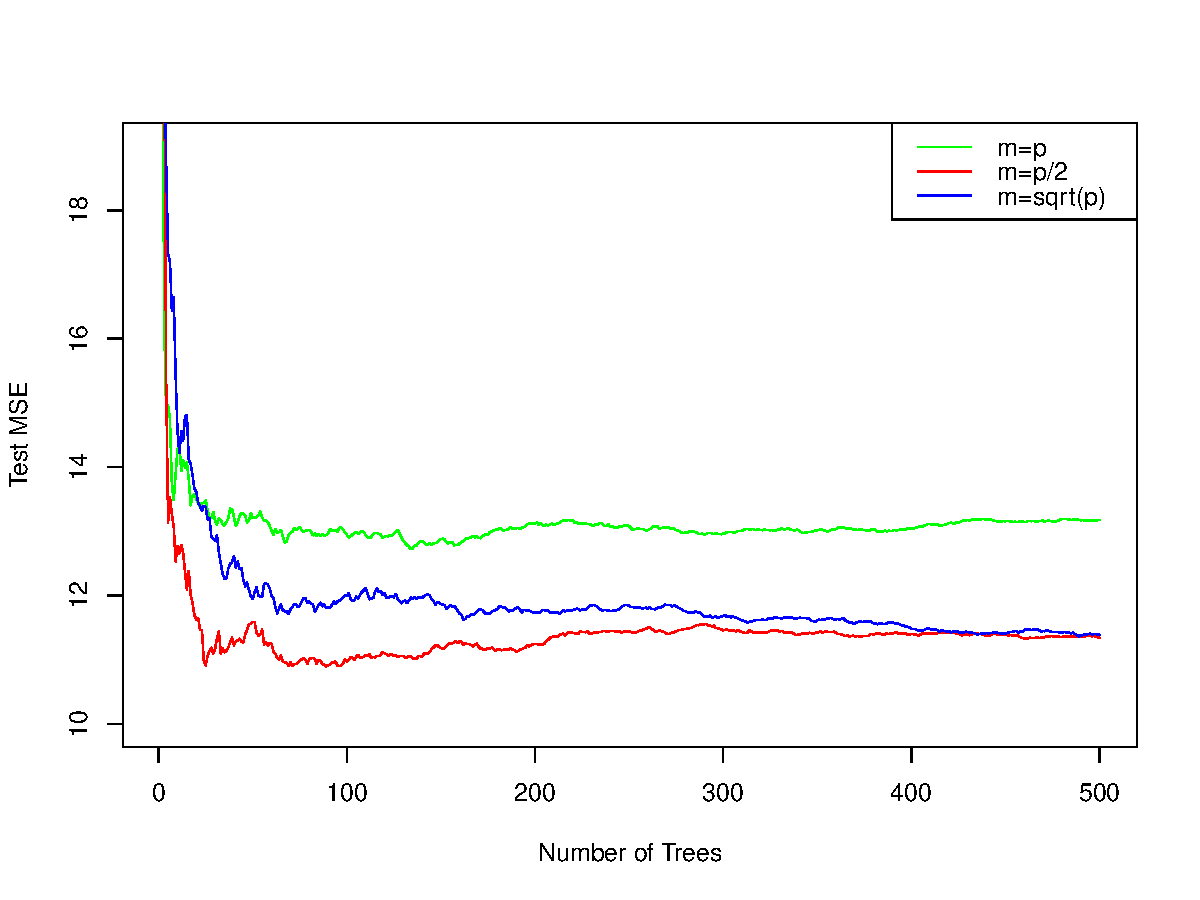
\includegraphics[width=0.8\textwidth]{MTH522_hw7_p1.pdf}
	\end{center}
	\caption{.}
	\label{fig:MTH522_hw7_p1}
\end{figure}
.\\
ntree: A range of ntree from 1 to 500.
From Plot: For single treee the "Test MSE" is very high like 19,but when number of tree increases  in the model the Test MSE drop down very quickly and after adding 100 trees to the model it stabilizes. \\
The Test MSE (m = p ,Green color) for all predictors is higher than other two of the number of predictors (m=p/2 and m=sqrt(p))


\newpage
{\bf Problem 2} (Chapter 8 Exercises 8):\\
In the lab, a classification tree was applied to the Carseats data set after converting Sales into a qualitative response variable. Now we will seek to predict Sales using regression trees and related approaches, treating the response as a quantitative variable.
(a) Split the data set into a training set and a test set.\\

\begin{program}
	\begin{verbatim}
	> library(ISLR)
	> attach(Carseats)
	> set.seed(1)
	> train = sample(dim(Carseats)[1], dim(Carseats)[1]/2)
	> Carseats.train = Carseats[train, ]
	> Carseats.test = Carseats[-train, ]
	\end{verbatim}
\end{program}

(b) Fit a regression tree to the training set. Plot the tree, and interpret the results. What test MSE do you obtain?\\

\begin{program}
	\begin{verbatim}
	> install.packages("tree")
	trying URL 'https://cran.cnr.berkeley.edu/bin/macosx/mavericks/contrib/3.3/tree_1.0-37.tgz'
	Content type 'application/x-gzip' length 112331 bytes (109 KB)
	==================================================
	downloaded 109 KB
	
	
	The downloaded binary packages are in
	/var/folders/28/5cht8_x964n2w_4_wf_1tn3m0000gn/T//Rtmpi5oCSV/downloaded_packages
	
	
	
	
	> library(tree)
	> tree.carseats = tree(Sales ~ ., data = Carseats.train)
	> summary(tree.carseats)
	
	Regression tree:
	tree(formula = Sales ~ ., data = Carseats.train)
	Variables actually used in tree construction:
	[1] "ShelveLoc"   "Price"       "Age"         "Advertising" "Income"      "CompPrice"  
	Number of terminal nodes:  18 
	Residual mean deviance:  2.36 = 429.5 / 182 
	Distribution of residuals:
	Min. 1st Qu.  Median    Mean 3rd Qu.    Max. 
	-4.2570 -1.0360  0.1024  0.0000  0.9301  3.9130 
	
	
	> plot(tree.carseats, cex = 0.2)
	> text(tree.carseats, pretty = 0, cex = 0.7)
	> dev.copy2pdf(file = "MTH522_hw7_p2a.pdf", width = 8, height = 6, out.type = "pdf")
	> dev.off()
	\end{verbatim}
\end{program}

\newpage

\begin{figure}[htb]
	\begin{center}
		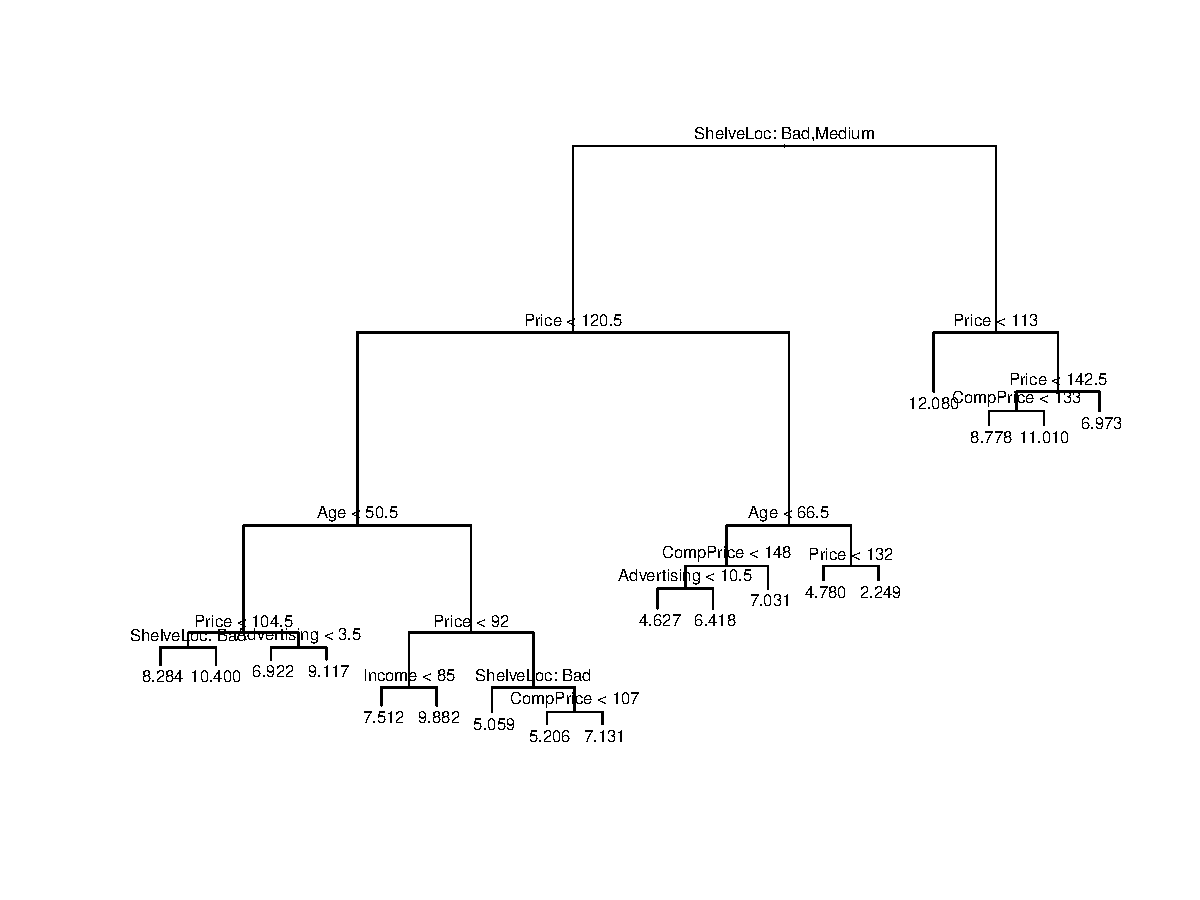
\includegraphics[width=0.8\textwidth]{MTH522_hw7_p2a.pdf}
	\end{center}
	\caption{.}
	\label{fig:MTH522_hw7_p2a}
\end{figure}

\begin{program}
	\begin{verbatim}
	> pred = predict(tree.carseats, Carseats.test)
	> mean((Carseats.test$Sales - pred)^2)
	
	[1] 4.148897
	\end{verbatim}
\end{program}

Result, Test MSE is 4.148897

\newpage

(c) Use cross-validation in order to determine the optimal level of tree complexity. Does pruning the tree improve the test MSE?\\

\begin{program}
	\begin{verbatim}
	> cv.carseats = cv.tree(tree.carseats)
	> plot(cv.carseats$size, cv.carseats$dev, type = "b")
	> dev.copy2pdf(file = "MTH522_hw7_p2c.pdf", width = 8, height = 6, out.type = "pdf")
\	> dev.off()
	\end{verbatim}
\end{program}

\begin{figure}[htb]
	\begin{center}
		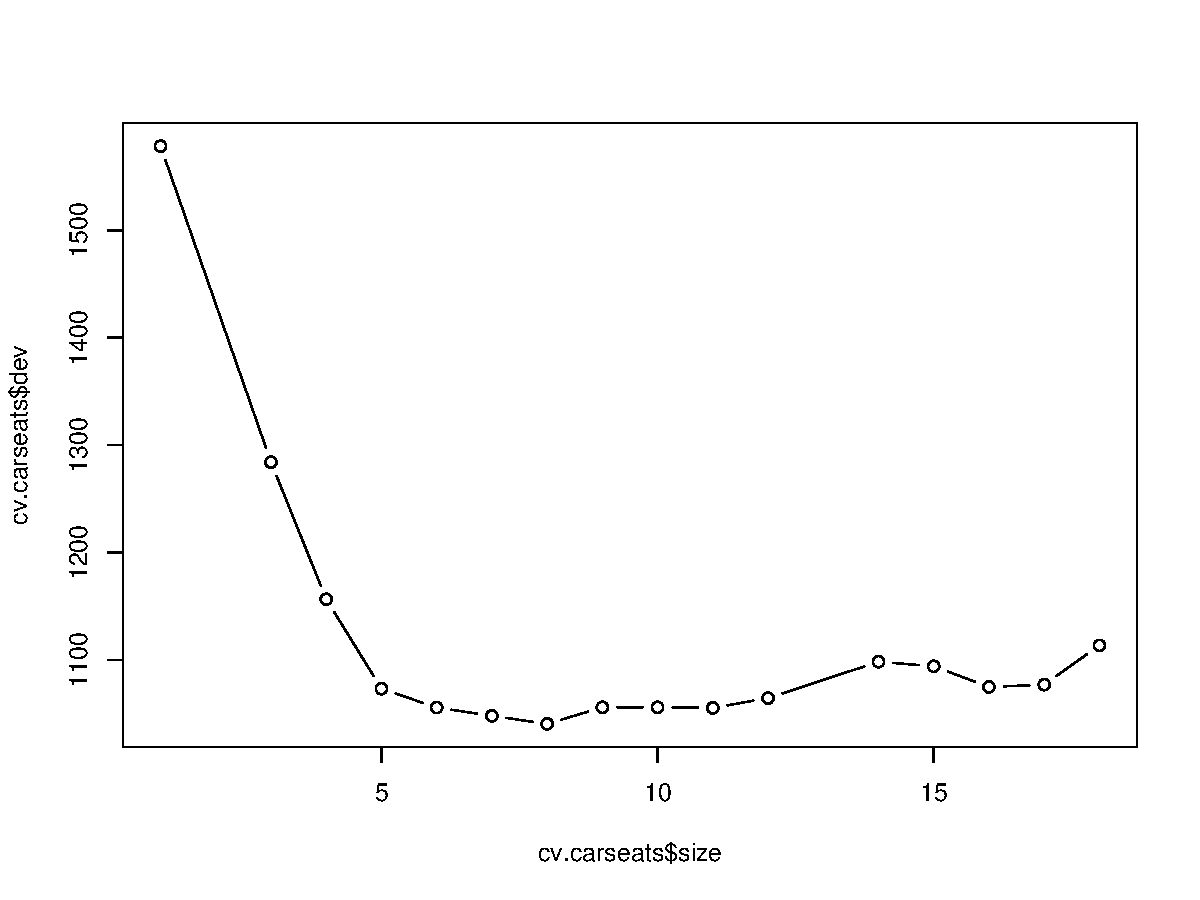
\includegraphics[width=0.8\textwidth]{MTH522_hw7_p2c.pdf}
	\end{center}
	\caption{.}
	\label{fig:MTH522_hw7_p2c}
\end{figure}

The tree of size 8 is selected by cross-validation. We now prune the tree to obtain the 8-node tree.\\

\newpage

\begin{program}
	\begin{verbatim}
	> pruned.carseats = prune.tree(tree.carseats, best = 8)
	> plot(pruned.carseats)
	> text(pruned.carseats, pretty = 0)
	> dev.copy2pdf(file = "MTH522_hw7_p2c_2.pdf", width = 8, height = 6, out.type = "pdf")
	> dev.off()
	\end{verbatim}
\end{program}

\begin{figure}[htb]
	\begin{center}
		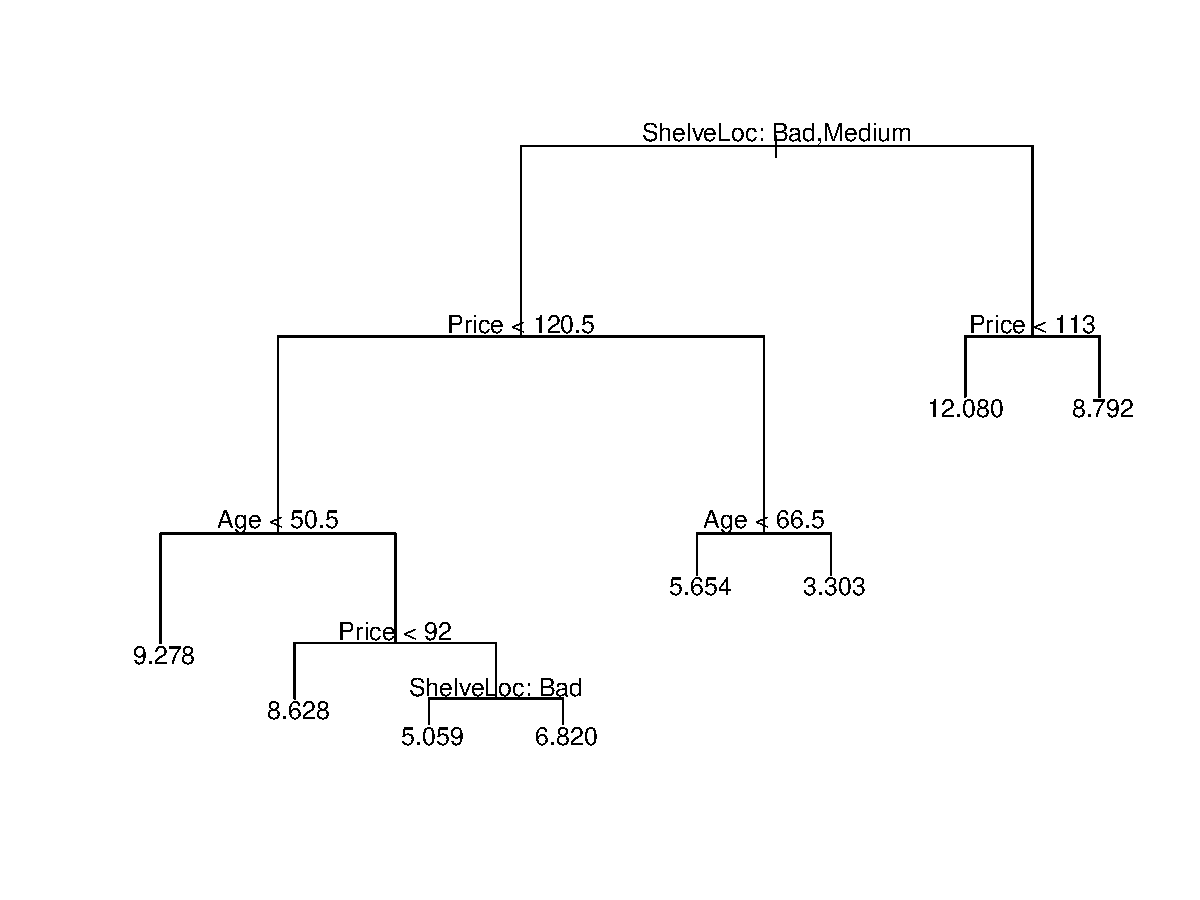
\includegraphics[width=0.8\textwidth]{MTH522_hw7_p2c_2.pdf}
	\end{center}
	\caption{.}
	\label{fig:MTH522_hw7_p2c_2}
\end{figure}

\begin{program}
	\begin{verbatim}
	> pred = predict(pruned.carseats, Carseats.test)
	> mean((Carseats.test$Sales - pred)^2)
	
	[1] 5.09085
	\end{verbatim}
\end{program}

We may say that pruning the tree increases the Test MSE to 5.09085.



\newpage

(d) Use the bagging approach in order to analyze this data. What test MSE do you obtain? Use the importance() function to determine which variables are most important.\\

\begin{program}
	\begin{verbatim}
	> library(randomForest)
	> carseats = randomForest(Sales ~ ., data = Carseats.train, mtry = 10, ntree = 500,
	+      importance = T)
	>  pred = predict(carseats, Carseats.test)
	>  mean((Carseats.test$Sales - pred)^2)
	
	[1] 2.583251
	\end{verbatim}
\end{program}


\begin{program}
	\begin{verbatim}
	> importance(bag.carseats)
	
	%IncMSE IncNodePurity
	CompPrice   13.06849545    130.785188
	Income       4.54737141     79.502339
	Advertising 13.53207401    131.998744
	Population   0.08549938     60.498175
	Price       57.10673896    504.769865
	ShelveLoc   43.30069615    320.415045
	Age         21.91388932    184.199205
	Education    2.50663690     40.334715
	Urban       -3.11593207      8.526444
	US           5.62400085     14.288796
	\end{verbatim}
\end{program}

We can say that bagging decrease the Test MSE error to 2.58.\\

"Price", "ShelveLoc" and "Age" are most important predictor veriables.
 
\newpage

(e) Use random forests to analyze this data. What test MSE do you obtain? Use the importance() function to determine which variables are most important. Describe the effect of m, the number of variables considered at each split, on the error rate obtained.


\begin{program}
	\begin{verbatim}
	> rf.carseats = randomForest(Sales ~ ., data = Carseats.train, mtry = 5, ntree = 500,
	+      importance = T)
	>  pred = predict(rf.carseats, Carseats.test)
	>  mean((pred - Carseats.test$Sales )^2)
	
	[1] 2.837792
	\end{verbatim}
\end{program}

\begin{program}
	\begin{verbatim}
	> importance(rf.carseats)
	%IncMSE IncNodePurity
	CompPrice   11.7995764     123.99149
	Income       4.5044593     109.90659
	Advertising 13.0146889     132.11725
	Population   2.0893802      84.74694
	Price       46.3418812     442.97829
	ShelveLoc   38.1022103     276.41698
	Age         17.7985501     199.49882
	Education    2.2709849      53.47066
	Urban        0.1619189      11.04973
	US           5.2523002      23.87314
	
	\end{verbatim}
\end{program}

We can say that random forest worsens the Test MSE error to 2.837792.\\

"Price", "ShelveLoc" and "Age" are still most important predictor veriables.

\newpage

{\bf Problem 3} (Chapter 8 Exercises 9):\\
This problem involves the OJ data set which is part of the ISLR package.\\
\begin{program}
	\begin{verbatim}
	> library(ISLR)
	> attach(OJ)
	> set.seed(1)
	> summary(OJ)
	
	Purchase WeekofPurchase     StoreID        PriceCH         PriceMM     
	CH:653   Min.   :227.0   Min.   :1.00   Min.   :1.690   Min.   :1.690  
	MM:417   1st Qu.:240.0   1st Qu.:2.00   1st Qu.:1.790   1st Qu.:1.990  
	Median :257.0   Median :3.00   Median :1.860   Median :2.090  
	Mean   :254.4   Mean   :3.96   Mean   :1.867   Mean   :2.085  
	3rd Qu.:268.0   3rd Qu.:7.00   3rd Qu.:1.990   3rd Qu.:2.180  
	Max.   :278.0   Max.   :7.00   Max.   :2.090   Max.   :2.290  
	DiscCH            DiscMM         SpecialCH        SpecialMM     
	Min.   :0.00000   Min.   :0.0000   Min.   :0.0000   Min.   :0.0000  
	1st Qu.:0.00000   1st Qu.:0.0000   1st Qu.:0.0000   1st Qu.:0.0000  
	Median :0.00000   Median :0.0000   Median :0.0000   Median :0.0000  
	Mean   :0.05186   Mean   :0.1234   Mean   :0.1477   Mean   :0.1617  
	3rd Qu.:0.00000   3rd Qu.:0.2300   3rd Qu.:0.0000   3rd Qu.:0.0000  
	Max.   :0.50000   Max.   :0.8000   Max.   :1.0000   Max.   :1.0000  
	LoyalCH          SalePriceMM     SalePriceCH      PriceDiff       Store7   
	Min.   :0.000011   Min.   :1.190   Min.   :1.390   Min.   :-0.6700   No :714  
	1st Qu.:0.325257   1st Qu.:1.690   1st Qu.:1.750   1st Qu.: 0.0000   Yes:356  
	Median :0.600000   Median :2.090   Median :1.860   Median : 0.2300            
	Mean   :0.565782   Mean   :1.962   Mean   :1.816   Mean   : 0.1465            
	3rd Qu.:0.850873   3rd Qu.:2.130   3rd Qu.:1.890   3rd Qu.: 0.3200            
	Max.   :0.999947   Max.   :2.290   Max.   :2.090   Max.   : 0.6400            
	PctDiscMM        PctDiscCH       ListPriceDiff       STORE      
	Min.   :0.0000   Min.   :0.00000   Min.   :0.000   Min.   :0.000  
	1st Qu.:0.0000   1st Qu.:0.00000   1st Qu.:0.140   1st Qu.:0.000  
	Median :0.0000   Median :0.00000   Median :0.240   Median :2.000  
	Mean   :0.0593   Mean   :0.02731   Mean   :0.218   Mean   :1.631  
	3rd Qu.:0.1127   3rd Qu.:0.00000   3rd Qu.:0.300   3rd Qu.:3.000  
	Max.   :0.4020   Max.   :0.25269   Max.   :0.440   Max.   :4.000  
	\end{verbatim}
\end{program}


(a) Create a training set containing a random sample of 800 observations, and a test set containing the remaining observations.\\

\begin{program}
	\begin{verbatim}
	> train = sample(dim(OJ)[1], 800)
	> OJ.train = OJ[train, ]
	> OJ.test = OJ[-train, ]
	\end{verbatim}
\end{program}


\newpage

(b) Fit a tree to the training data, with Purchase as the response and the other variables except for Buy as predictors. Use the summary() function to produce summary statistics about the tree, and describe the results obtained. What is the training error rate? How many terminal nodes does the tree have?\\

\begin{program}
	\begin{verbatim}
	> library(tree)
	> oj.tree = tree(Purchase ~ ., data = OJ.train)
	> summary(oj.tree)
	
	Classification tree:
	tree(formula = Purchase ~ ., data = OJ.train)
	Variables actually used in tree construction:
	[1] "LoyalCH"       "PriceDiff"     "SpecialCH"     "ListPriceDiff"
	Number of terminal nodes:  8 
	Residual mean deviance:  0.7305 = 578.6 / 792 
	Misclassification error rate: 0.165 = 132 / 800 
	\end{verbatim}
\end{program}

The tree uses variables  are  "LoyalCH", "PriceDiff",  "SpecialCH", "ListPriceDiff" and  has 8 terminal nodes and a misclassification (training) error rate of 0.165.\\

(c) Type in the name of the tree object in order to get a detailed text output. Pick one of the terminal nodes, and interpret the information displayed.\\

\begin{program}
	\begin{verbatim}
	> oj.tree
	
	
	node), split, n, deviance, yval, (yprob)
	* denotes terminal node
	
	1) root 800 1064.00 CH ( 0.61750 0.38250 )  
	2) LoyalCH < 0.508643 350  409.30 MM ( 0.27143 0.72857 )  
	4) LoyalCH < 0.264232 166  122.10 MM ( 0.12048 0.87952 )  
	8) LoyalCH < 0.0356415 57   10.07 MM ( 0.01754 0.98246 ) *
	9) LoyalCH > 0.0356415 109  100.90 MM ( 0.17431 0.82569 ) *
	5) LoyalCH > 0.264232 184  248.80 MM ( 0.40761 0.59239 )  
	10) PriceDiff < 0.195 83   91.66 MM ( 0.24096 0.75904 )  
	20) SpecialCH < 0.5 70   60.89 MM ( 0.15714 0.84286 ) *
	21) SpecialCH > 0.5 13   16.05 CH ( 0.69231 0.30769 ) *
	11) PriceDiff > 0.195 101  139.20 CH ( 0.54455 0.45545 ) *
	3) LoyalCH > 0.508643 450  318.10 CH ( 0.88667 0.11333 )  
	6) LoyalCH < 0.764572 172  188.90 CH ( 0.76163 0.23837 )  
	12) ListPriceDiff < 0.235 70   95.61 CH ( 0.57143 0.42857 ) *
	13) ListPriceDiff > 0.235 102   69.76 CH ( 0.89216 0.10784 ) *
	7) LoyalCH > 0.764572 278   86.14 CH ( 0.96403 0.03597 ) *
	\end{verbatim}
\end{program}

The asterisk (*) in the line shows that it is a terminal node.
I picked terminal node label 9. The splitting value of this node is 0.0356415. There are 109 subtree below this node with deviance of 100.9. The prediction at this node is Sales = MM. About  17.431\% of the observations in this node take the value of CH and remaining 82.569\% take the value of MM.


\newpage


(d) Create a plot of the tree, and interpret the results.\\

\begin{program}
	\begin{verbatim}
		> plot(oj.tree, cex = 0.2)
		> text(oj.tree, pretty = 0, cex = 0.7)
		> dev.copy2pdf(file = "MTH522_hw7_p3d.pdf", width = 8, height = 6, out.type = "pdf")
		> dev.off()
		
	\end{verbatim}
\end{program}

\begin{figure}[htb]
	\begin{center}
		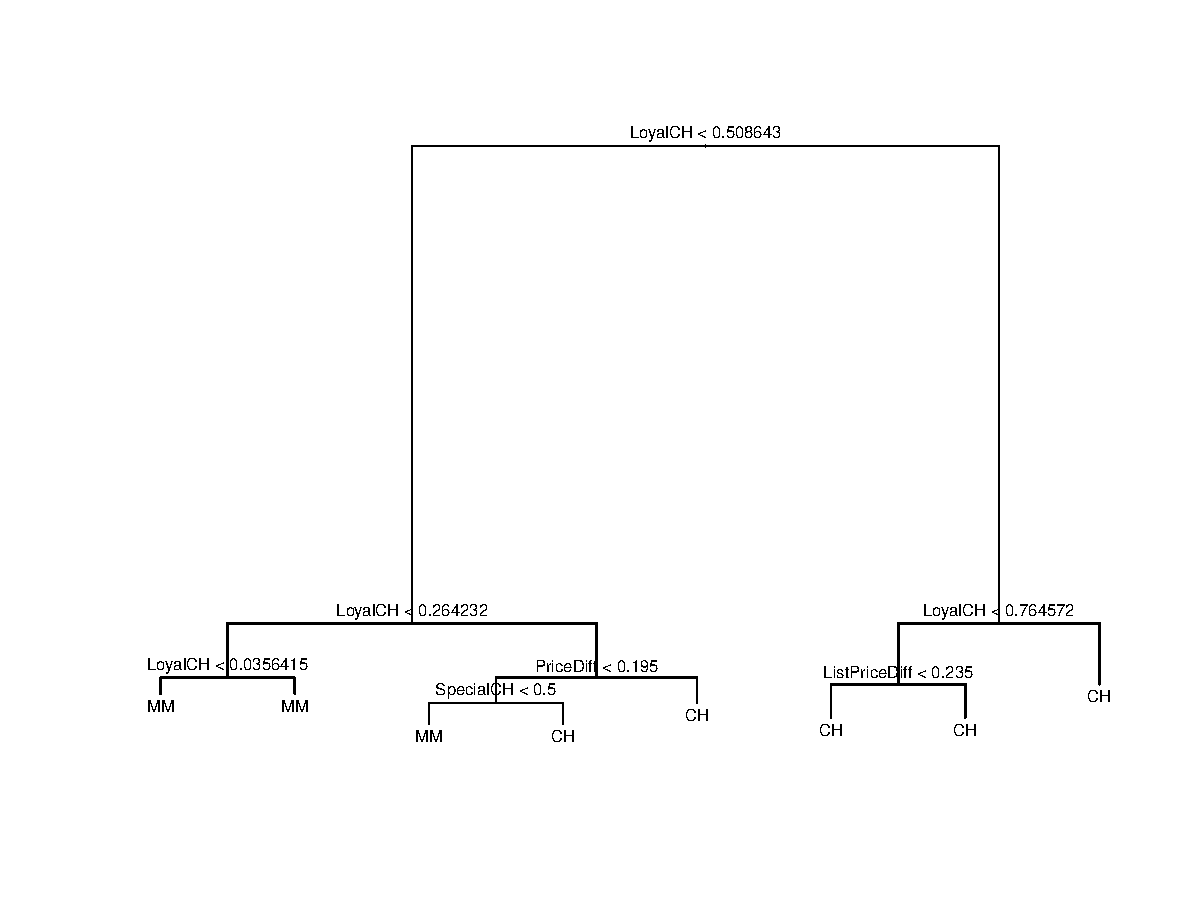
\includegraphics[width=0.8\textwidth]{MTH522_hw7_p3d.pdf}
	\end{center}
	\caption{.}
	\label{fig:MTH522_hw7_p3d}
\end{figure}

"LoyalCH" is the most important indicator of tree. The top three nodes contain "LoyalCH". If  "LoyalCH" < 0.264243, the tree predicts MM. If  "LoyalCH" => 0.764572, the tree predicts CH. Between those values of "LoyalCH", the decision depends  on the value of "PriceDiff" and "ListPriceDiff"

\newpage


(e) Predict the response on the test data, and produce a confusion matrix comparing the test labels to the predicted test labels. What is the test error rate?\\

\begin{program}
	\begin{verbatim}
	> oj.pred = predict(oj.tree, OJ.test, type = "class")
	> table(OJ.test$Purchase, oj.pred)
	
	
	oj.pred
	CH  MM
	CH 147  12
	MM  49  62
	
	
	
	
	> 1 - (147 + 62) / (147+12+49+62)
	[1] 0.2259259
	\end{verbatim}
\end{program}

Test error rate : 0.2259259


(f) Apply the cv.tree() function to the training set in order to determine the optimal tree size.\\

\begin{program}
	\begin{verbatim}
	> cv.oj = cv.tree(oj.tree, FUN = prune.tree)
	> cv.oj


	$size
	[1] 8 7 6 5 4 3 2 1
	
	$dev
	[1]  689.1001  685.8030  654.9314  653.7774  666.8890  721.2494  733.6936 1066.6499
	
	$k
	[1]      -Inf  11.20965  14.72877  17.88334  23.55203  38.37537  43.02529 337.08200
	
	$method
	[1] "deviance"
	
	attr(,"class")
	[1] "prune"         "tree.sequence"
	
	\end{verbatim}
\end{program}


\newpage


(g) Produce a plot with tree size on the x-axis and cross-validated classification error rate on the y-axis.\\

\begin{program}
	\begin{verbatim}
	> plot(cv.oj$size, cv.oj$dev, type = "b", xlab = "Tree Size", ylab = "Deviance")
	> dev.copy2pdf(file = "MTH522_hw7_p3g.pdf", width = 8, height = 6, out.type = "pdf")
	> dev.off()
	\end{verbatim}
\end{program}

\begin{figure}[htb]
	\begin{center}
		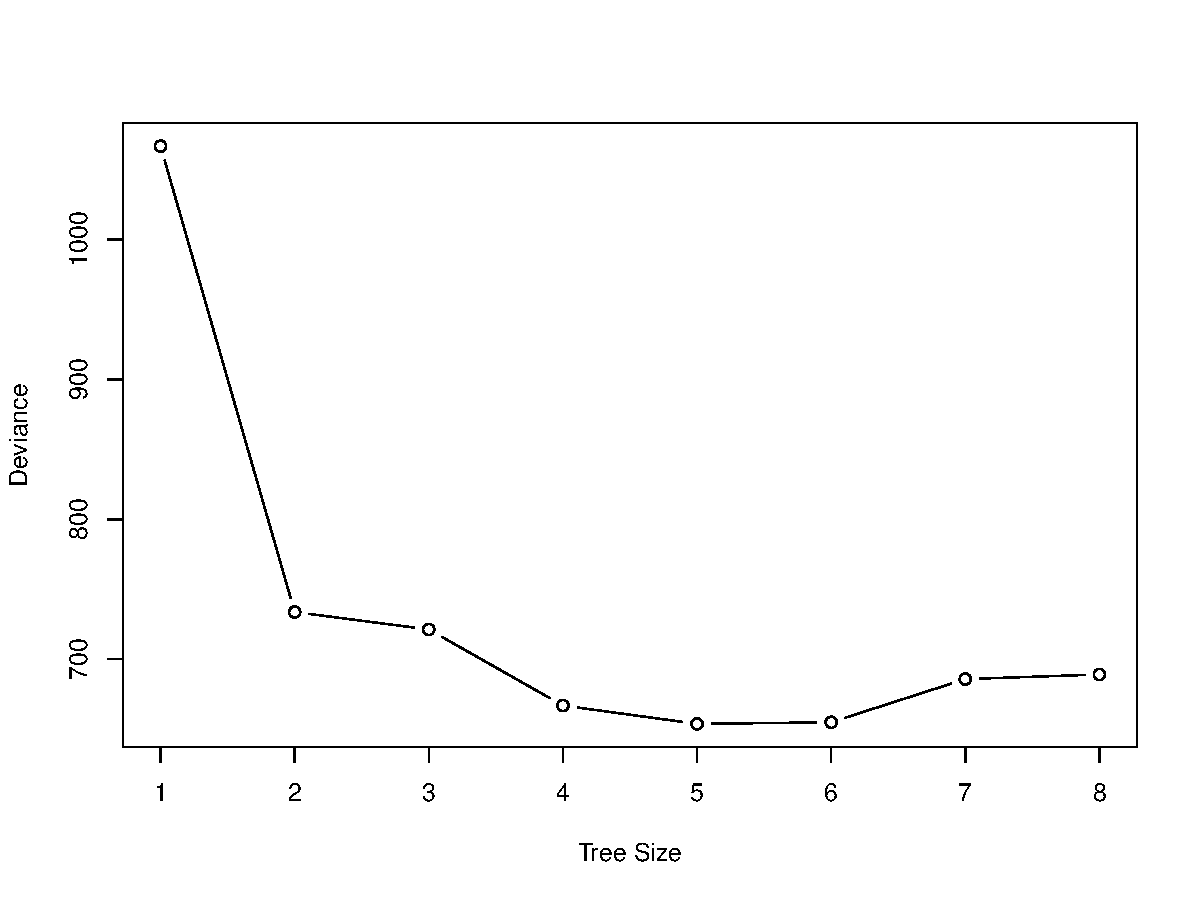
\includegraphics[width=0.8\textwidth]{MTH522_hw7_p3g.pdf}
	\end{center}
	\caption{.}
	\label{fig:MTH522_hw7_p3g}
\end{figure}




(h) Which tree size corresponds to the lowest cross-validated classi- fication error rate?\\

\begin{program}
	\begin{verbatim}
	The 5-node tree is the smallest tree with the lowest cross-validation error rate.
	\end{verbatim}
\end{program}


\newpage


(i) Produce a pruned tree corresponding to the optimal tree size obtained using cross-validation. If cross-validation does not lead to selection of a pruned tree, then create a pruned tree with five terminal nodes.\\

\begin{program}
	\begin{verbatim}
	> oj.prune = prune.tree(oj.tree, best = 5)
	> plot(oj.prune)
	> text(oj.prune, pretty = 0)
	> dev.copy2pdf(file = "MTH522_hw7_p3i.pdf", width = 8, height = 6, out.type = "pdf")
	> dev.off()
	\end{verbatim}
\end{program}

\begin{figure}[htb]
	\begin{center}
		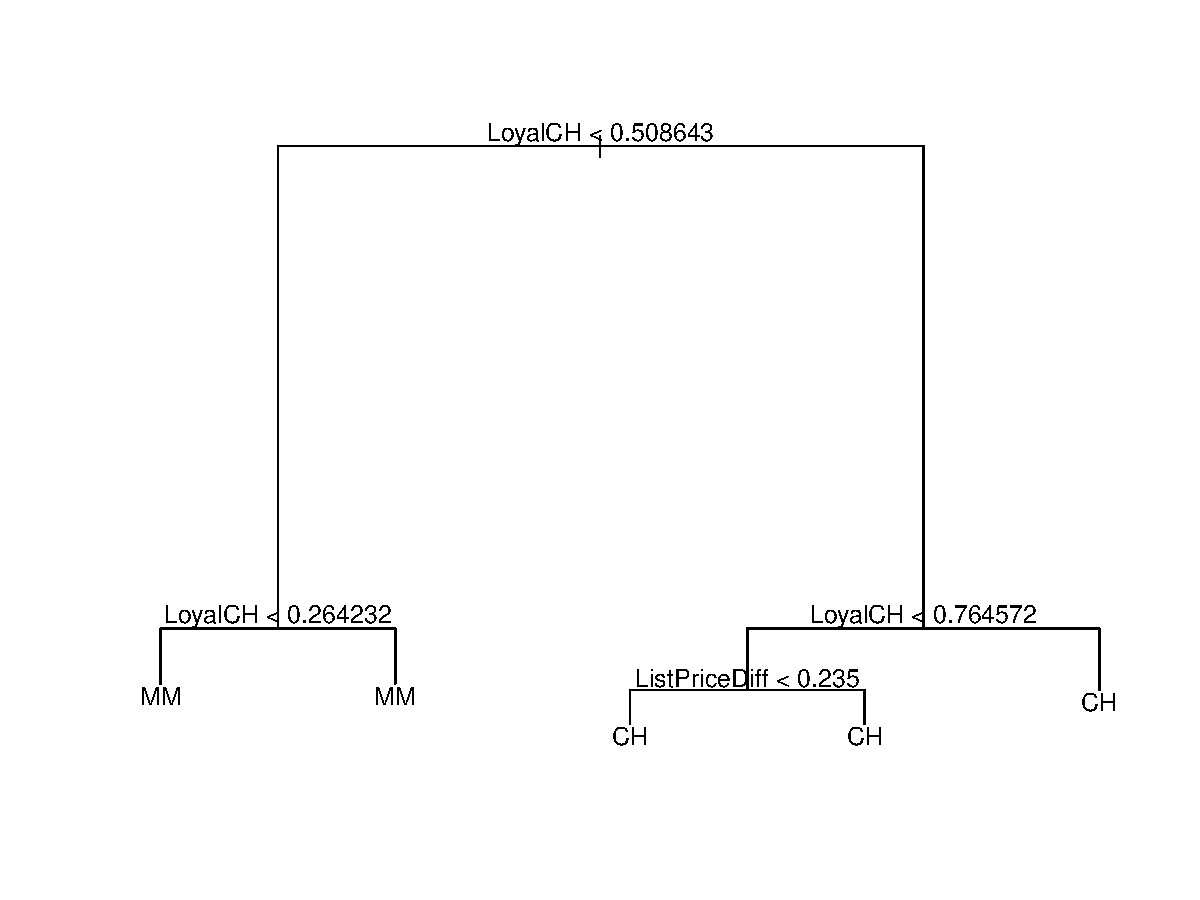
\includegraphics[width=0.8\textwidth]{MTH522_hw7_p3i.pdf}
	\end{center}
	\caption{.}
	\label{fig:MTH522_hw7_p3i}
\end{figure}


\newpage

(j) Compare the training error rates between the pruned and un- pruned trees. Which is higher?\\

\begin{program}
	\begin{verbatim}
	> summary(oj.tree)
	
	
	Classification tree:
	tree(formula = Purchase ~ ., data = OJ.train)
	Variables actually used in tree construction:
	[1] "LoyalCH"       "PriceDiff"     "SpecialCH"     "ListPriceDiff"
	Number of terminal nodes:  8 
	Residual mean deviance:  0.7305 = 578.6 / 792 
	Misclassification error rate: 0.165 = 132 / 800 
	
	> summary(oj.prune)
	
	Classification tree:
	snip.tree(tree = oj.tree, nodes = 4:5)
	Variables actually used in tree construction:
	[1] "LoyalCH"       "ListPriceDiff"
	Number of terminal nodes:  5 
	Residual mean deviance:  0.7829 = 622.4 / 795 
	Misclassification error rate: 0.1825 = 146 / 800 	
	\end{verbatim}
\end{program}

Misclassification error of prune tree (0.1825) is slightly higher than original treel tree (0.165). \\




(k) Compare the test error rates between the pruned and unpruned trees. Which is higher?\\

\begin{program}
	\begin{verbatim}
	> pred.unprune = predict(oj.tree, OJ.test, type = "class")
	> table(pred.unprune, OJ.test$Purchase)
	
	pred.unprune  CH  MM
	CH 147  49
	MM  12  62
	
	> 1 - (147+62) / (147+49+12+62)
	[1] 0.2259259
	
	
	> pred.prune = predict(oj.prune, OJ.test, type = "class")
	> table(pred.prune, OJ.test$Purchase)
	
	pred.prune  CH  MM
	CH 119  30
	MM  40  81
	
	> 1 - (119 + 81) / (119+30+40+81)
	[1] 0.2592593
	\end{verbatim}
\end{program}

Prune test error rate 0.2592593 is slightly higher than unpruned trees error rate of 0.2259259 .



\newpage
{\bf Problem 4} (Chapter 8 Exercises 10):\\
We now use boosting to predict Salary in the Hitters data set.\\

\begin{program}
	\begin{verbatim}
	> library(ISLR)
	> summary(Hitters)
	AtBat            Hits         HmRun            Runs             RBI        
	Min.   : 16.0   Min.   :  1   Min.   : 0.00   Min.   :  0.00   Min.   :  0.00  
	1st Qu.:255.2   1st Qu.: 64   1st Qu.: 4.00   1st Qu.: 30.25   1st Qu.: 28.00  
	Median :379.5   Median : 96   Median : 8.00   Median : 48.00   Median : 44.00  
	Mean   :380.9   Mean   :101   Mean   :10.77   Mean   : 50.91   Mean   : 48.03  
	3rd Qu.:512.0   3rd Qu.:137   3rd Qu.:16.00   3rd Qu.: 69.00   3rd Qu.: 64.75  
	Max.   :687.0   Max.   :238   Max.   :40.00   Max.   :130.00   Max.   :121.00  
	
	Walks            Years            CAtBat            CHits            CHmRun      
	Min.   :  0.00   Min.   : 1.000   Min.   :   19.0   Min.   :   4.0   Min.   :  0.00  
	1st Qu.: 22.00   1st Qu.: 4.000   1st Qu.:  816.8   1st Qu.: 209.0   1st Qu.: 14.00  
	Median : 35.00   Median : 6.000   Median : 1928.0   Median : 508.0   Median : 37.50  
	Mean   : 38.74   Mean   : 7.444   Mean   : 2648.7   Mean   : 717.6   Mean   : 69.49  
	3rd Qu.: 53.00   3rd Qu.:11.000   3rd Qu.: 3924.2   3rd Qu.:1059.2   3rd Qu.: 90.00  
	Max.   :105.00   Max.   :24.000   Max.   :14053.0   Max.   :4256.0   Max.   :548.00  
	
	CRuns             CRBI             CWalks        League  Division
	Min.   :   1.0   Min.   :   0.00   Min.   :   0.00   A:175   E:157   
	1st Qu.: 100.2   1st Qu.:  88.75   1st Qu.:  67.25   N:147   W:165   
	Median : 247.0   Median : 220.50   Median : 170.50                   
	Mean   : 358.8   Mean   : 330.12   Mean   : 260.24                   
	3rd Qu.: 526.2   3rd Qu.: 426.25   3rd Qu.: 339.25                   
	Max.   :2165.0   Max.   :1659.00   Max.   :1566.00                   
	
	PutOuts          Assists          Errors          Salary       NewLeague
	Min.   :   0.0   Min.   :  0.0   Min.   : 0.00   Min.   :  67.5   A:176    
	1st Qu.: 109.2   1st Qu.:  7.0   1st Qu.: 3.00   1st Qu.: 190.0   N:146    
	Median : 212.0   Median : 39.5   Median : 6.00   Median : 425.0            
	Mean   : 288.9   Mean   :106.9   Mean   : 8.04   Mean   : 535.9            
	3rd Qu.: 325.0   3rd Qu.:166.0   3rd Qu.:11.00   3rd Qu.: 750.0            
	Max.   :1378.0   Max.   :492.0   Max.   :32.00   Max.   :2460.0            
	NA's   :59                
	\end{verbatim}
\end{program}

(a) Remove the observations for whom the salary information is unknown, and then log-transform the salaries.\\

\begin{program}
	\begin{verbatim}
	> Hitters = na.omit(Hitters)
	> Hitters$Salary = log(Hitters$Salary)
	\end{verbatim}
\end{program}


\newpage

(b) Create a training set consisting of the first 200 observations, and a test set consisting of the remaining observations. \\

\begin{program}
	\begin{verbatim}
	> train = 1:200
	>  Hitters.train = Hitters[train, ]
	>  Hitters.test = Hitters[-train, ]
	\end{verbatim}
\end{program}

(c) Perform boosting on the training set with 1,000 trees for a range of values of the shrinkage parameter λ. Produce a plot with different shrinkage values on the x-axis and the corresponding training set MSE on the y-axis. \\

\begin{program}
	\begin{verbatim}
	> install.packages("gbm")
	--- Please select a CRAN mirror for use in this session ---
	trying URL 'https://cran.cnr.berkeley.edu/bin/macosx/mavericks/contrib/3.3/gbm_2.1.1.tgz'
	Content type 'application/x-gzip' length 853908 bytes (833 KB)
	==================================================
	downloaded 833 KB
	
	
	The downloaded binary packages are in
	/var/folders/28/5cht8_x964n2w_4_wf_1tn3m0000gn/T//RtmpMqMQ7L/downloaded_packages
	\end{verbatim}
\end{program}

\begin{program}
	\begin{verbatim}
	> library(gbm)
	Loading required package: survival
	Loading required package: lattice
	Loading required package: splines
	Loading required package: parallel
	Loaded gbm 2.1.1
	
	> set.seed(1)
	>  pows = seq(-10, -0.2, by = 0.1)
	>  lambdas = 10^pows
	>  length.lambdas = length(lambdas)
	>  train.errors = rep(NA, length.lambdas)
	>  test.errors = rep(NA, length.lambdas)
	>  for (i in 1:length.lambdas) {
	+      boost.hitters = gbm(Salary ~ ., data = Hitters.train, distribution = "gaussian",
	+          n.trees = 1000, shrinkage = lambdas[i])
	+      train.pred = predict(boost.hitters, Hitters.train, n.trees = 1000)
	+      test.pred = predict(boost.hitters, Hitters.test, n.trees = 1000)
	+      train.errors[i] = mean((Hitters.train$Salary - train.pred)^2)
	+      test.errors[i] = mean((Hitters.test$Salary - test.pred)^2)
	+ }
	>  plot(lambdas, train.errors, type = "b", xlab = "Shrinkage", ylab = "Train MSE",
	+      col = "blue", pch = 20)
	> dev.copy2pdf(file = "MTH522_hw7_p4c.pdf", width = 8, height = 6, out.type = "pdf")
	> dev.off() 
	\end{verbatim}
\end{program}


\begin{figure}[htb]
	\begin{center}
		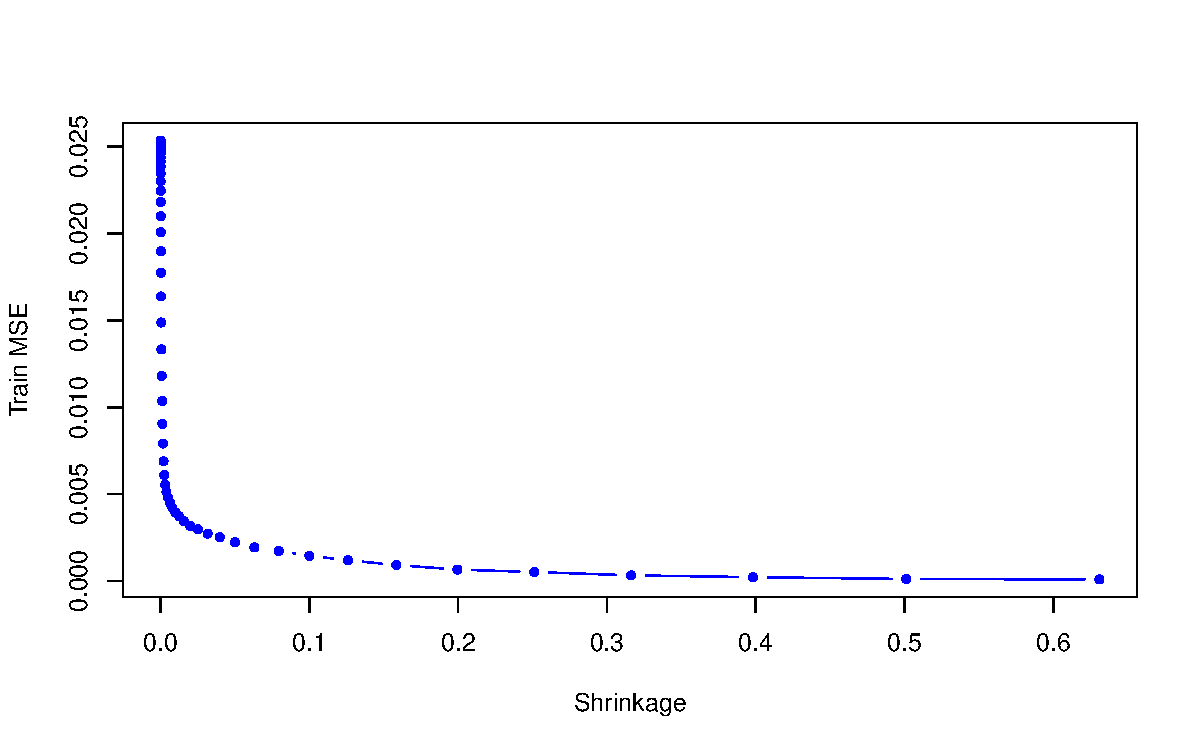
\includegraphics[width=0.8\textwidth]{MTH522_hw7_p4c.pdf}
	\end{center}
	\caption{.}
	\label{fig:MTH522_hw7_p4c}
\end{figure}

\newpage


(d) Produce a plot with different shrinkage values on the x-axis and the corresponding test set MSE on the y-axis. \\

\begin{program}
	\begin{verbatim}
	> plot(lambdas, test.errors, type = "b", xlab = "Shrinkage", ylab = "Test MSE")
	> dev.copy2pdf(file = "MTH522_hw7_p4d.pdf", width = 8, height = 6, out.type = "pdf")
	> dev.off()
	\end{verbatim}
\end{program}

\begin{figure}[htb]
	\begin{center}
		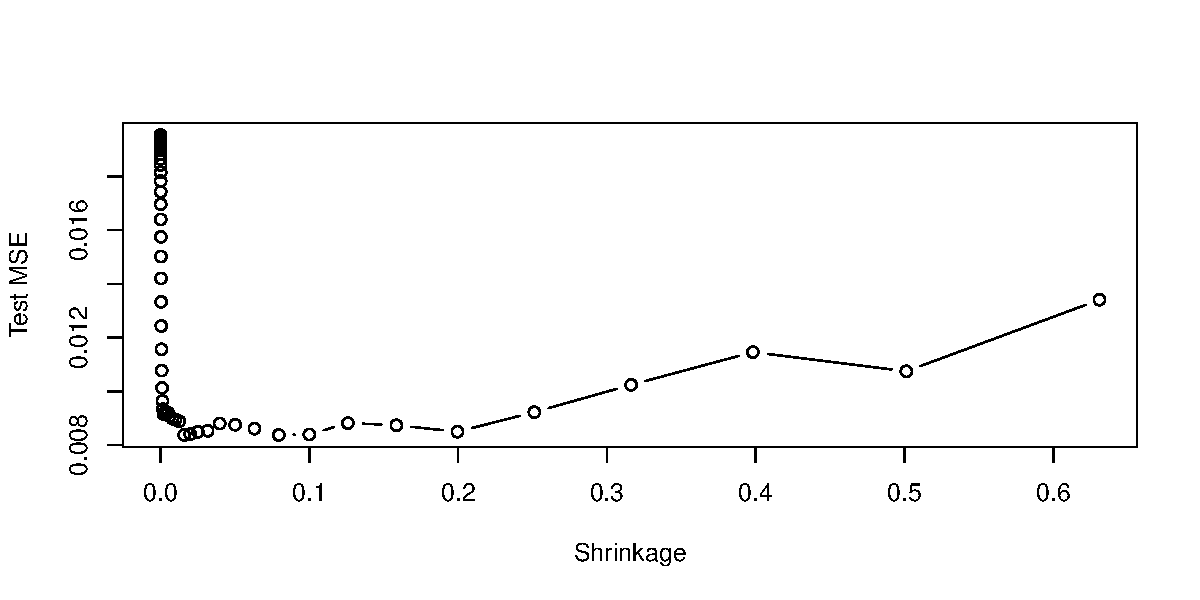
\includegraphics[width=0.8\textwidth]{MTH522_hw7_p4d.pdf}
	\end{center}
	\caption{.}
	\label{fig:MTH522_hw7_p4d}
\end{figure}

\newpage

\begin{program}
	\begin{verbatim}
	> min(test.errors)
	[1] 0.008371305
	> 
	> lambdas[which.min(test.errors)]
	[1] 0.07943282
	\end{verbatim}
\end{program}
The minimum test MSE is 0.008371305, and is obtained for $\lambda$ = 0.07943282.\\


(e) Compare the test MSE of boosting to the test MSE that results from applying two of the regression approaches seen in Chapters 3 and 6. \\

\begin{program}
	\begin{verbatim}
	>   library(glmnet)
	Loading required package: Matrix
	Loading required package: foreach
	foreach: simple, scalable parallel programming from Revolution Analytics
	Use Revolution R for scalability, fault tolerance and more.
	http://www.revolutionanalytics.com
	Loaded glmnet 2.0-5
	
	
	> lm.fit = lm(Salary ~ ., data = Hitters.train)
	> lm.pred = predict(lm.fit, Hitters.test)
	> mean((Hitters.test$Salary - lm.pred)^2)
	[1] 0.01496996
	
	
	> set.seed(1)
	> x = model.matrix(Salary ~ ., data = Hitters.train)
	> y = Hitters.train$Salary
	> x.test = model.matrix(Salary ~ ., data = Hitters.test)
	> lasso.fit = glmnet(x, y, alpha = 1)
	> lasso.pred = predict(lasso.fit, s = 0.01, newx = x.test)
	> mean((Hitters.test$Salary - lasso.pred)^2)
	[1] 0.01377199
	\end{verbatim}
\end{program}

The linear regression and ridge regression have higher test MSE than boostong.


\newpage


(f) Which variables appear to be the most important predictors in the boosted model? \\

\begin{program}
	\begin{verbatim}
	> library(gbm)
	> boost.best = gbm(Salary ~ ., data = Hitters.train, distribution = "gaussian",
	+     n.trees = 1000, shrinkage = lambdas[which.min(test.errors)])
	> summary(boost.best)
	var     rel.inf
	CAtBat       CAtBat 16.39917007
	CRBI           CRBI 12.00135571
	CRuns         CRuns  9.66158055
	PutOuts     PutOuts  7.82936035
	CHits         CHits  7.69734758
	Walks         Walks  6.90002087
	Years         Years  5.49896314
	CWalks       CWalks  5.48705226
	RBI             RBI  5.07463775
	AtBat         AtBat  4.22862860
	Assists     Assists  3.86031219
	CHmRun       CHmRun  3.67125349
	HmRun         HmRun  2.93359813
	Hits           Hits  2.81299263
	Runs           Runs  2.47761436
	Errors       Errors  2.21998496
	NewLeague NewLeague  0.58142871
	Division   Division  0.56870414
	League       League  0.09599453

	> dev.copy2pdf(file = "MTH522_hw7_p4f.pdf", width = 8, height = 4, out.type = "pdf")
	> dev.off()
		\end{verbatim}
\end{program}

“CAtBat”  and "CRBI" are two most important variables in that order.

\begin{figure}[htb]
	\begin{center}
		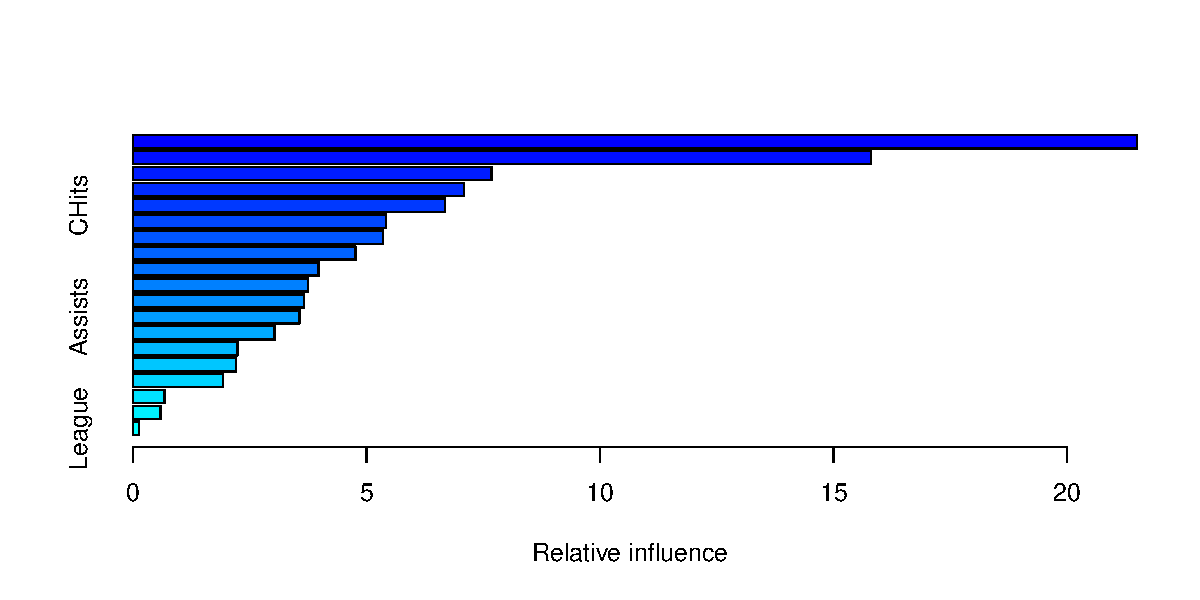
\includegraphics[width=0.8\textwidth]{MTH522_hw7_p4f.pdf}
	\end{center}
	\caption{.}
	\label{fig:MTH522_hw7_p4f}
\end{figure}


\newpage


(g) Now apply bagging to the training set. What is the test set MSE for this approach? \\

\begin{program}
	\begin{verbatim}
	> set.seed(1)
	>  rf.hitters = randomForest(Salary ~ ., data = Hitters.train, ntree = 500, mtry = 19)
	>  rf.pred = predict(rf.hitters, Hitters.test)
	>  mean((Hitters.test$Salary - rf.pred)^2)
	
	[1] 0.007368052
	\end{verbatim}
\end{program}

Test MSE for bagging is about 0.0074 , which is slightly lower than the best test MSE for boosting.


\newpage
{\bf Problem 5} (Chapter 8 Exercises 12):\\
Apply boosting, bagging, and random forests to a data set of your choice. Be sure to fit the models on a training set and to evaluate their performance on a test set. How accurate are the results compared to simple methods like linear or logistic regression? Which of these approaches yields the best performance? \\
\\

I will use “Weekly” data set for this question.

\begin{program}
	\begin{verbatim}
	> library(ISLR)
	> set.seed(1)
	> summary(Weekly)
	
	Year           Lag1               Lag2               Lag3         
	Min.   :1990   Min.   :-18.1950   Min.   :-18.1950   Min.   :-18.1950  
	1st Qu.:1995   1st Qu.: -1.1540   1st Qu.: -1.1540   1st Qu.: -1.1580  
	Median :2000   Median :  0.2410   Median :  0.2410   Median :  0.2410  
	Mean   :2000   Mean   :  0.1506   Mean   :  0.1511   Mean   :  0.1472  
	3rd Qu.:2005   3rd Qu.:  1.4050   3rd Qu.:  1.4090   3rd Qu.:  1.4090  
	Max.   :2010   Max.   : 12.0260   Max.   : 12.0260   Max.   : 12.0260  
	Lag4               Lag5              Volume            Today          Direction 
	Min.   :-18.1950   Min.   :-18.1950   Min.   :0.08747   Min.   :-18.1950   Down:484  
	1st Qu.: -1.1580   1st Qu.: -1.1660   1st Qu.:0.33202   1st Qu.: -1.1540   Up  :605  
	Median :  0.2380   Median :  0.2340   Median :1.00268   Median :  0.2410             
	Mean   :  0.1458   Mean   :  0.1399   Mean   :1.57462   Mean   :  0.1499             
	3rd Qu.:  1.4090   3rd Qu.:  1.4050   3rd Qu.:2.05373   3rd Qu.:  1.4050             
	Max.   : 12.0260   Max.   : 12.0260   Max.   :9.32821   Max.   : 12.0260             
	\end{verbatim}
\end{program}


\begin{program}
	\begin{verbatim}
	> train = sample(nrow(Weekly), nrow(Weekly)/2)
	> test = -train
	\end{verbatim}
\end{program}

LOGISTIC REGRESSION

\begin{program}
	\begin{verbatim}
	> glm.fit = glm(Direction ~ . - Year - Today, data = Weekly[train, ],
	+ family = "binomial")
	> glm.probs = predict(glm.fit, newdata = Weekly[test, ], type =
	+ "response")
	> glm.pred = rep("Down", length(glm.probs))
	> glm.pred[glm.probs > 0.5] = "Up"
	> table(glm.pred, Weekly$Direction[test])
	
	glm.pred Down  Up
	Down   28  32
	Up    225 260


	> 1 - (28+260) / (28+32+225+260)
	[1] 0.4715596
	\end{verbatim}
\end{program}

Error : 0.4715596

\newpage

BOOSTING


\begin{program}
	\begin{verbatim}
	> library(gbm)
	> Weekly$BinomialDirection = ifelse(Weekly$Direction == "Up", 1, 0)
	> boost.weekly = gbm(BinomialDirection ~ . - Year - Today - Direction,
	+ data = Weekly[train,
	+     ], distribution = "bernoulli", n.trees = 5000)
	> yhat.boost = predict(boost.weekly, newdata = Weekly[test, ], n.trees
	+ = 5000)
	> yhat.pred = rep(0, length(yhat.boost))
	> yhat.pred[yhat.boost > 0.5] = 1
	> table(yhat.pred, Weekly$BinomialDirection[test])
	
	yhat.pred   0   1
	0 204 221
	1  49  71


	> 1 - (204+71) / (204+221+49+71)
	[1] 0.4954128
	\end{verbatim}
\end{program}

Error : 0.4954128 \\

BAGGING

\begin{program}
	\begin{verbatim}
	> Weekly = Weekly[, !(names(Weekly) %in% c("BinomialDirection"))]
	> library(randomForest)
	> bag.weekly = randomForest(Direction ~ . - Year - Today, data =
	+ Weekly, subset = train,
	+     mtry = 6)
	> yhat.bag = predict(bag.weekly, newdata = Weekly[test, ])
	> table(yhat.bag, Weekly$Direction[test])
	
	yhat.bag Down  Up
	Down   82  81
	Up    171 211


	> 1 - (82+211)/(82+81+171+211)
	[1] 0.4623853
	\end{verbatim}
\end{program}

Error : 0.4623853 \\

\newpage

RANDOM FORESTS

\begin{program}
	\begin{verbatim}
	> rf.weekly = randomForest(Direction ~ . - Year - Today, data =
	+ Weekly, subset = train,
	+     mtry = 2)
	> yhat.bag = predict(rf.weekly, newdata = Weekly[test, ])
	> table(yhat.bag, Weekly$Direction[test])
	
	yhat.bag Down  Up
	Down   68  73
	Up    185 219



	> 1 - (68+219)/(68+73+185+219)
	[1] 0.4733945
	\end{verbatim}
\end{program}

Error : 0.4733945 \\

BAGGING gave th lowest validation set test error rate.



\end{document}





